% !TEX encoding = IsoLatin
\documentclass[slidetop,11pt]{beamer}
\usetheme{Frankfurt}
\usepackage[T1]{fontenc} 
\usepackage[latin1]{inputenc} 
\usepackage[french]{babel}
\usepackage{pslatex}
\usepackage{tikz}
\usepackage{graphics}
\usetikzlibrary{shapes}
\usepackage{multicol}

\author{Guillaume BOUR}
\title{Reconnaissance optique de caract�res manuscrits}
\subtitle{Application � la reconnaissance de codes postaux}

\date{\textsc{Juillet 2016}} 

\setbeamertemplate{navigation symbols}{}
\setbeamertemplate{caption}{\raggedright\insertcaption\par}


\begin{document}


% DIAPO 1
\begin{frame}
    \titlepage
\end{frame}


% DIAPO 2
\begin{frame}
    \frametitle{Sommaire}
    \tableofcontents
\end{frame}

\section{Introduction}

\section{Pr�sentation g�n�rale d'un OCR}

\subsection*{D�finition et domaines d'application d'un OC}


%DIAPO 3
\begin{frame} 
    \frametitle{D�finition et domaines d'application d'un OCR}
    
    \begin{block}{Optical Character Recognition}
    Un logiciel OCR est un programme qui � partir d'une image num�rique (scan, photo...) produit en sortie un fichier de texte avec le texte reconnu.
    \end{block}
    
    \vspace{0.5cm}
    \hspace*{-0.5cm}
    \begin{tikzpicture}
    \node[inner sep=0pt] (russell) at (0,0)
        {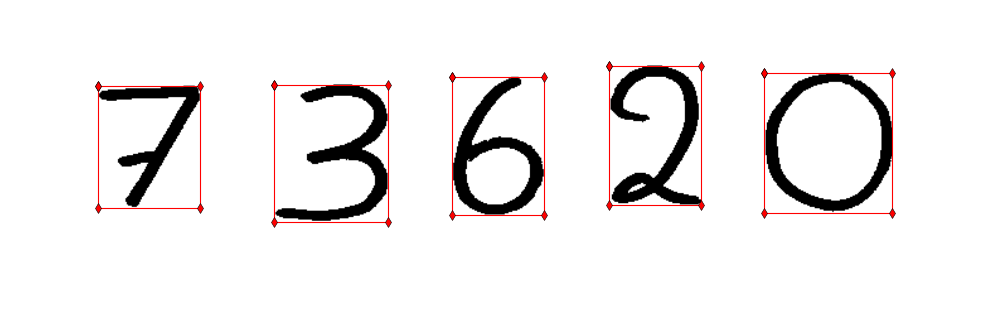
\includegraphics[width=.50\textwidth]{img/73620_characters.png}};
    \node[inner sep=0pt] (whitehead) at (6,-2)
        {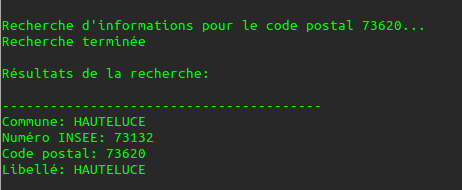
\includegraphics[width=.5\textwidth]{img/hauteluce_reconnu.png}};
    \draw[->,>=latex] (russell.south) |- (whitehead.west)
        node[midway,fill=white] {\tiny Programme de reconnaissance};
    \end{tikzpicture}
\end{frame}

\subsection*{Objectif du programme}


%DIAPO 4
\begin{frame} 
    \frametitle{Objectif du programme}
    
    \hspace*{-0.7cm}
    \begin{minipage}[c]{0.45\textwidth}
    \begin{figure}
    \centering
    \fbox{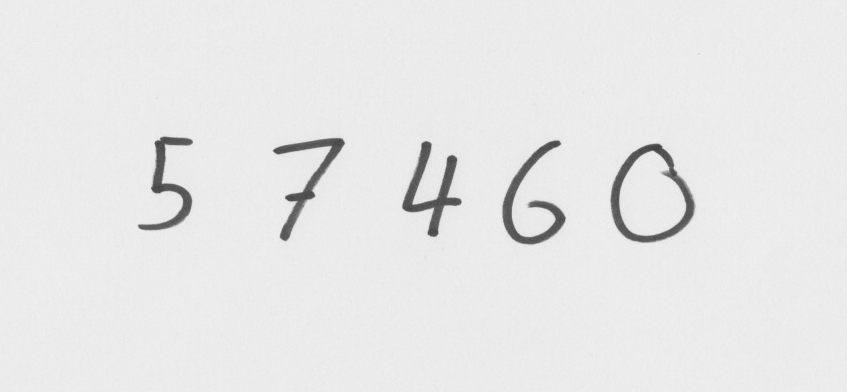
\includegraphics[width=5cm]{img/code_57460_light.png}}
    \caption{\footnotesize Exemple d'entr�e du programme}
    \end{figure}
    \end{minipage}\hfill
    \begin{minipage}{0.45\textwidth}
    \begin{figure}
    \centering
    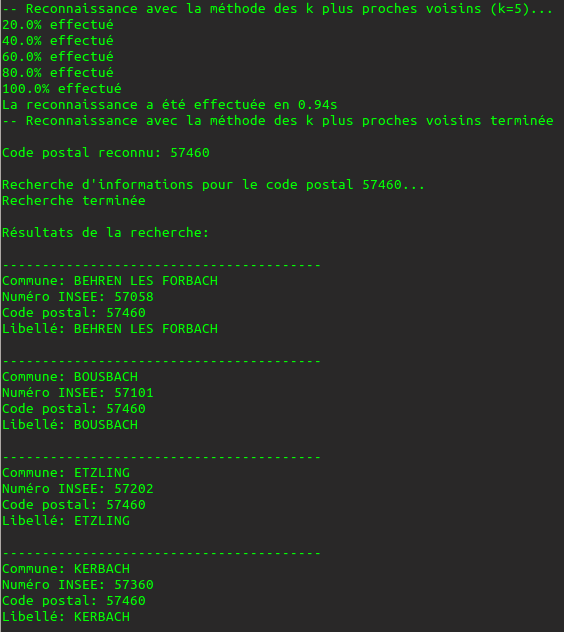
\includegraphics[width=5cm]{img/execution_Programme.png}
    \caption{\footnotesize R�sultat de l'ex�cution}
    \end{figure}
    \end{minipage}
\end{frame}

\section{Algorithme de reconnaissance}

\subsection*{Fonctionnement et �tapes du programme}


% DIAPO 5
\begin{frame} 
    \frametitle{Fonctionnement et �tapes du programme \hfill\scriptsize p. 4 � 8}
    \vspace{-0.5cm}   
    \begin{center}
    \hspace*{-0.3cm}
    
    \begin{tikzpicture}
    \node[draw,minimum height=0.5cm,rounded corners=3pt, fill = lightgray, text centered] (D) at(-1,2.5) { Fonctionnement du programme};
    
    \node[draw] (P) at (-5,0) {Pr�-analyse};
    \node[draw] (S) at (-3,-2) {Segmentation};
    \node[draw] (R) at (0,0) {Reconnaissance};
    \node[draw] (T) at (3,-2) {Post-Traitement};
    \draw[->,>=latex] (P) |- (S);
    \draw[->,>=latex] (S) |- (R);
    \draw[->,>=latex] (R) |- (T);
    
    \node[draw,minimum height=1cm,dashed,text width=3cm, text centered] (D) at(-5,1) {{\scriptsize Seuillage, d�tection des contours}};
    \node[draw,minimum height=1cm,dashed,text width=3cm, text centered] (D) at(-3,-3) {{\scriptsize Isolation des chiffres, normalisation}};
    \node[draw,minimum height=1cm,dashed,text width=3cm, text centered] (D) at(0,1) {{\scriptsize Classification avec kNN}};
    \node[draw,minimum height=1cm,dashed,text width=3cm, text centered] (D) at(3,-3) {{\scriptsize Cross-validation, BDD}};
    \end{tikzpicture}
    
    \end{center}
\end{frame}

\subsection*{Algorithme kNN (k-Nearest Neighbours)}


% DIAPO 6
\begin{frame} 
    \frametitle{Algorithme kNN (k-Nearest Neighbours) \hfill\scriptsize p. 5 - 7 - 30}
    
    \begin{block}{Pr�sentation}
    La m�thode des \textbf{k plus proches voisins} (kNN) est une m�thode d'apprentissage supervis�e qui permet, � partir d'une base de donn�es d'apprentissage, d'estimer la valeur d'une nouvelle entr�e.
    \end{block}
    
    \begin{figure}
    \begin{minipage}[c]{0.55\linewidth}
    \fbox{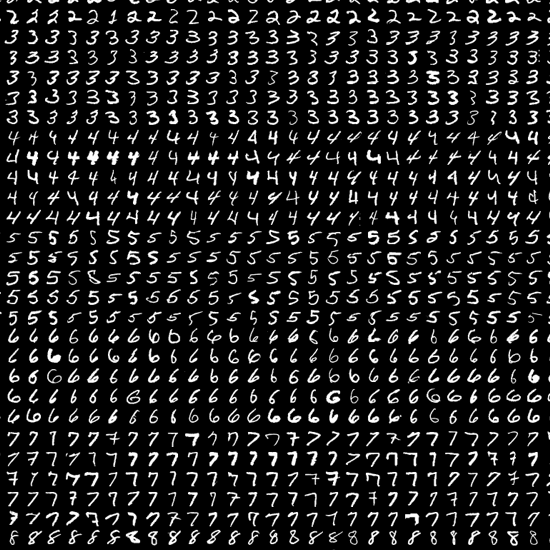
\includegraphics[width=5cm]{img/digits_crop.png}}
    \end{minipage}
    \begin{minipage}[c]{0.35\linewidth}
    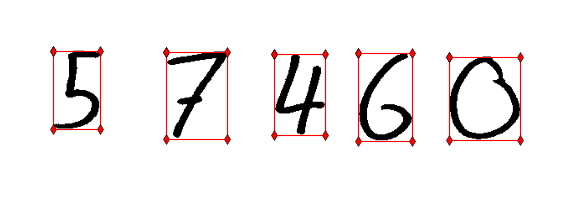
\includegraphics[width=4.5cm]{img/exemple_code_postal.png}
    \end{minipage}
    \end{figure}
\end{frame}


% DIAPO 7
\begin{frame} 
    \frametitle{Algorithme kNN (k-Nearest Neighbours) \hfill\scriptsize p. 29 - 30}
    
    \begin{block}{Distance Euclidienne}
    \scriptsize
    $S = \{0,1\}$, 
    $M_1, M_2 \in \mathcal{M}_n(S)$
    \vspace{-0.5cm}
    $$d_E(M_1,M_2) = \sqrt{\sum_{i=0}^n \sum_{j=0}^n (m_{1_{i,j}}-m_{2_{i,j}})^2}$$
    \end{block}
    
    \begin{center}
    \scalebox{0.90}{
    \begin{tikzpicture}
    
    \node[draw, circle, fill=red!50] (I) at (0,0) {{\tiny ?}};
    
    \draw[dashed] (0,0) circle (1.5);
    \draw[dotted] (0,0) circle (2.5);
    
    \node[draw, rectangle, fill=green!50] (I) at (0.3,1) {{\tiny 4}};
    \node[draw, rectangle, fill=green!50] (I) at (-1,-0.5) {{\tiny 4}};
    \node[draw, rectangle, fill=green!50] (I) at (-1.5,2.5) {{\tiny 4}};
    
    \node[draw, rectangle, fill=blue!50] (I) at (0.5,-0.5) {{\tiny 5}};
    \node[draw, rectangle, fill=blue!50] (I) at (2,0.5) {{\tiny 5}};
    \node[draw, rectangle, fill=blue!50] (I) at (0.5,-1.8) {{\tiny 5}};
    
    \node[draw, rectangle, fill=green!50] (I) at (-2.5,2.3) {{\tiny 4}};
    \node[draw, rectangle, fill=green!50] (I) at (-3,0.5) {{\tiny 4}};
    
    \node[draw, rectangle, fill=blue!50] (I) at (2,-2) {{\tiny 5}};
    \node[draw, rectangle, fill=blue!50] (I) at (3,-1) {{\tiny 5}};
    
    \node[draw] (K) at (0,1.8) {{\tiny k = 3}};
    \node[draw] (K) at (0,2.8) {{\tiny k = 5}};
    
    
    \node[draw,minimum height=0.5cm,rounded corners=3pt, text centered] (D) at(0,-3) {Classification d'une nouvelle entr�e};
    
    \end{tikzpicture}}
    \end{center}
\end{frame}


\section{Am�lioration de l'efficacit�}

\subsection*{Utilisation d'une m�thode de validation crois�e}


% DIAPO 8
\begin{frame}
    \frametitle{Utilisation d'une m�thode de validation crois�e \hfill\scriptsize p. 31 - 32}
    \framesubtitle{Principe}
    
    \begin{tikzpicture}
    \node[inner sep=0pt] (russell) at (0,0)
        {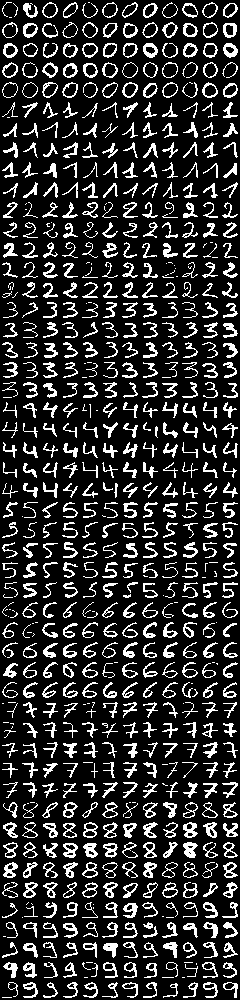
\includegraphics[width=.15\textwidth]{img/image_test.png}};
    \node[inner sep=0pt] (whitehead) at (8,0)
        {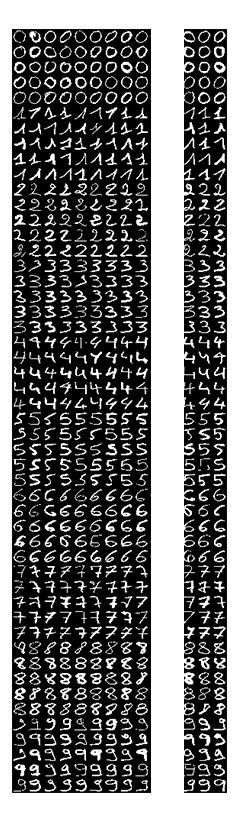
\includegraphics[width=.20\textwidth]{img/crossValidationIllustration.png}};
    \draw[->,thick] (russell.east) -- (whitehead.west)
        node[midway,fill=white] {\tiny S�paration de l'�chantillon};
        
    \node[draw] (un) at (7.6,-3.75) {\tiny75\%};
    \node[draw] (deux) at (8.75,-3.75) {\tiny25\%};
    
    \node[draw] (zero) at (0,-3.75) {\tiny Echantillon de r�f�rence};
    
    \end{tikzpicture}
\end{frame}


% DIAPO 9
\begin{frame} 
    \frametitle{Utilisation d'une m�thode de validation crois�e  \hfill\scriptsize p. 31 - 32}
    \framesubtitle{R�sultats}
    
    \begin{minipage}{\linewidth}
    \centering
    \hspace*{-0.3cm}
    \begin{tikzpicture}
    [xscale=0.16,yscale=0.06]
    \draw (0,0) grid[xstep = 5, ystep = 10] (65,90);
    \draw[gray,very thin] (0,0) grid[xstep=5,ystep=5] (65,90);
    \draw[line width=1mm,color=blue!50] plot[ycomb] file {data/crossValidationHoldoutResult_pourcentage.txt};
    \foreach \y in {5,10,15,...,90} \draw(0,\y)node[left]{\tiny{\y}};
    \foreach \x in {0,5,10,...,65} \draw(\x,0)node[below]{\tiny{\x}};
    \draw (4,92) node[above] {{\tiny Proportion reconnue (\%)}};
    \draw (66,0) node[right] {\footnotesize k};
    \node[draw] (T) at (32.5,-13) {\footnotesize\textsc{Estimation du pourcentage de caract�res reconnus en fonction de k}};
    
    \draw[line width=1mm,color=red!50] plot[ycomb] coordinates {(5,86.66)};
    
    \end{tikzpicture}
    \end{minipage}
\end{frame}


\subsection*{Utilisation d'une base de donn�es}


% DIAPO 10
\begin{frame} 
    \frametitle{Utilisation d'une base de donn�es  \hfill\scriptsize p. 30 - 34}
    \framesubtitle{Gestion des incertitudes}
    
    \hspace*{-0.5cm}
    \begin{minipage}[c]{0.30\linewidth}
    \begin{center}
    {\scriptsize Structure de la table \textbf{villes\_francaises}}\\
    \vspace{0.5cm}
    \begin{tabular}{|c|}
    \hline
    villes\_francaises \\
    \hline
    \tiny{id (pk)} \\
    \tiny{nom\_commune}\\
    \tiny{code\_commune\_INSEE}\\
    \tiny{code\_postal}\\
    \tiny{libelle\_acheminement}\\
    \tiny{ligne\_5}\\
    \hline
    \end{tabular}
    \end{center}
    \end{minipage}\hfill
    \begin{minipage}[c]{0.68\linewidth}
    \centering
    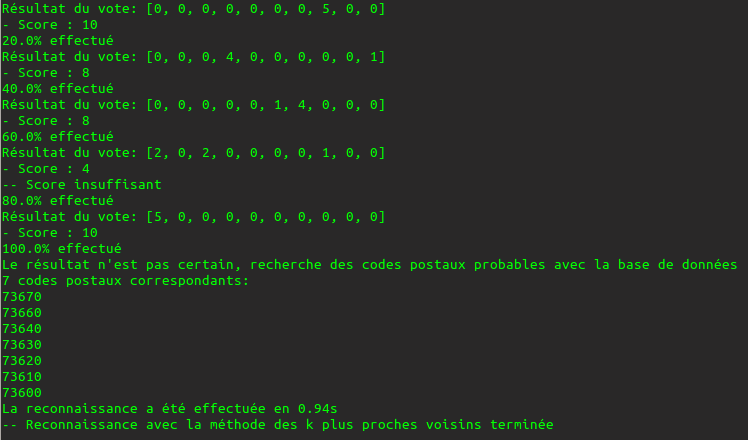
\includegraphics[width=7cm]{img/scores_DB.png}\\
    
    \tiny R�sultats dans le cas d'une recherche <<incertaine>>
    \end{minipage}
\end{frame}


\section{Conclusion}


% DIAPO 11
\begin{frame}
    \frametitle{Conclusion}
    
    \textsc{Bibliographie}
    
    \begin{itemize}
    \item Internet :
    	\begin{itemize}
       	\item Olivier Bernard, cours sur le Traitement d'images num�riques, INSA Lyon
       	\item OpenCV source code  \url{https://github.com/Itseez/opencv}
    	\end{itemize}
    \item Livres :
    	\begin{itemize}
       	\item Scott Krig, Computer Vision Metrics, Apress, 2014
       	\item Andrew R. Webb, Keith D. Copsey, Statistical Pattern Recognition, 3rd edition, Wiley, 2011
       	\item T. Y. Zhang, C. Y. Suen, A Fast Parallel Algorithm for thinning digital patterns, 1984
    	\end{itemize}
    \end{itemize}
\end{frame}

\end{document}